\documentclass[12pt]{article}
\usepackage[a4paper, margin=1in]{geometry} 
\usepackage{graphicx} 
\usepackage{hyperref}
\usepackage{float}
\usepackage{multicol}
\usepackage{multirow}
\usepackage{amsmath}
\usepackage[ruled]{algorithm2e}
\usepackage{amssymb}
\usepackage[font=small, labelfont=bf]{caption}
\usepackage[table,xcdraw]{xcolor}

\title{Lecture Notes for \\ INF281 Basics of Bioinformatics Sequence Analysis}
\author{Takaya Saito}
\date{}

\begin{document}

\pagenumbering{arabic}
\setcounter{page}{73}

\makeatletter 
\renewcommand{\thefigure}{\arabic{section}.\arabic{figure}}
\renewcommand{\thetable}{\arabic{section}.\arabic{table}}
\makeatother

%
% Progressive alignment
%
\setcounter{section}{9}
\setcounter{figure}{0}
\setcounter{table}{0}
\section{Progressive alignment}
%\documentclass[12pt]{article}
%\usepackage[a4paper, margin=1in]{geometry} 
%\usepackage{graphicx} 
%\usepackage{hyperref}
%\usepackage{float}
%\usepackage{multicol}
%\usepackage{multirow}
%\usepackage{amsmath}
%\usepackage[font=small, labelfont=bf]{caption}
%
%\begin{document}

%
% Introduction to progressive alignment
%
\subsection{Introduction to progressive alignment}
Several heuristic solutions to compute MSAs have been developed to avoid the multi-dimensional DP approach that requires heavy computational power.

%
% Three cases of aligning multiple sequences
%
\subsubsection*{Three cases of aligning multiple sequences}
\begin{itemize}
\item Two sequences, e.g. $s^1$ and $s^2$
\item One alignment and one sequence, e.g. $\mathcal{A}^1$ and $s^1$
\item Two alignments, e.g. $\mathcal{A}^1$ and $\mathcal{A}^2$
\end{itemize}

%
% Guiding methods
%
\subsubsection*{Guiding methods}
\begin{itemize}
\item Clustering
\item Phylogenetic tree
\end{itemize}

%
% Aligning methods
%
\subsubsection*{Aligning methods}
\begin{itemize}
\item Complete alignment
\item Pair-guided alignment
\end{itemize}

%
% Once a gap always a gap
%
\subsubsection*{Once a gap always a gap}
Many progressive alignment procedures use the “once a gap always a gap” policy, hence it is difficult to fix the errors that are made in early steps.

\bigskip 

%\end{document}

%\documentclass[12pt]{article}
%\usepackage[a4paper, margin=1in]{geometry} 
%\usepackage{graphicx} 
%\usepackage{hyperref}
%\usepackage{float}
%\usepackage{multicol}
%\usepackage{multirow}
%\usepackage{amsmath}
%\usepackage{amssymb}
%\usepackage[ruled]{algorithm2e}
%\usepackage[font=small, labelfont=bf]{caption}
%
%\begin{document}

%
% Alignment clustering
%
\subsection{Alignment clustering}
Alignment clustering can be used even when accurate phylogenic trees are not available. 

%
% Clustering methods
%
\subsubsection*{Clustering methods}
\begin{itemize}
\item Linear clustering
\item Linkage clustering
\end{itemize}

%
% Linear clustering
%
\subsubsection*{Linear clustering}
\begin{enumerate}
\item Start with an alignment with a single sequence
\item Add a single sequence to the alignment
\item Repeat until no sequence is left
\end{enumerate}

%
% Selection of the next sequence
%
\subsubsection*{Selection of the next sequence}
\begin{itemize}
\item Most similar to the one already in the alignment
\item Most similar to the average sequence in the alignment
\end{itemize}

%
% Pseudo-code of linear progressive alignment (general progressive alignment)
%
\subsubsection*{Pseudo-code of linear progressive alignment (general progressive alignment)}

\begin{algorithm}[H]
  \SetKwInOut{U}{$\mathrm{U}$}
  \SetKwInOut{A}{$\mathrm{A}$}
  \SetKwData{dRAB}{$\mathrm{R_{a,b}}$}
  \SetKwData{dG}{$\mathrm{g}$}
  
  \BlankLine
    
  \U{Set of sequences not aligned}
  \A{Current alignment}
  
  \BlankLine \BlankLine
  
   $\mathrm{U} \leftarrow \{s_1, s_2, ... s_n\}$;\\
   Choose two sequences s and t from U;\\
   $\mathrm{U} \leftarrow \mathrm{U} - \{s, t\}$;\\
   $\mathrm{A} \leftarrow Align(s, t)$;

  \BlankLine \BlankLine

  \For{$i \leftarrow 1$ \KwTo $n-2$}{
      Choose a sequence s from U;\\
      $\mathrm{U} \leftarrow \mathrm{U} - \{s\}$;\\
      $\mathrm{A} \leftarrow Align(\mathrm{A}, s)$;
  }

  \SetAlgoRefName{\thesection.1}
  \caption{General progressive alignment}

\end{algorithm}

%
% Linkage methods
%
\subsubsection*{Linkage methods}
It requires the pair-wise alignment scores of all possible combinations. 

\begin{itemize}
\item Average linkage
\item Maximum linkage
\item Minimum linkage
\end{itemize}

%
% Example of linkage methods
%
\subsubsection*{Example of linkage methods}
It requires the pair-wise alignment scores of all possible combinations. \\

\noindent
Decide two alignments from the three alignments, $\mathrm{A}^1 = \{s^1\}, \mathrm{A}^2 = \{s^2\}$, and $\mathrm{A}^3 = \{s^3, s^4\}$, for clustering.\\

Pair-wise scores

\begin{table}[H]
\centering
\begin{tabular}{|l|l|l|l|l|}
\hline
   & s1 & s2 & s3 & s4 \\ \hline
s1 & 0  & 7  & 5  & 3  \\ \hline
s2 &    & 0  & 4  & 8  \\ \hline
s3 &    &    & 0  & 2  \\ \hline
s4 &    &    &    & 0  \\ \hline
\end{tabular}
\end{table}

%
% NEWPAGE
%
\newpage

Linkage selection

\begin{table}[H]
\centering
\begin{tabular}{lll}
Average linkage & $S(\mathrm{A}_1,\mathrm{A}_2) = 7$               & \checkmark  \\
                & $S(\mathrm{A}_1,\mathrm{A}_3) = (5+3)/2 = 4$       &   \\
                & $S(\mathrm{A}_2,\mathrm{A}_3) = (4+8)/2 = 6$       &   \\
                &                                                            &   \\
Maximum linkage & $S(\mathrm{A}_1, \mathrm{A}_2) = 7$               &   \\
                & $S(\mathrm{A}_1, \mathrm{A}_3) = \max(5, 3) = 5$ &   \\
                & $S(\mathrm{A}_2, \mathrm{A}_3) = \max(4, 8) = 8$   & \checkmark \\
                &                                                            &   \\
Minimum linkage & $S(\mathrm{A}_1, \mathrm{A}_2) = 7$               & \checkmark \\
                & $S(\mathrm{A}_1, \mathrm{A}_3 ) = \min(5, 3) = 3$ &   \\
                & $S(\mathrm{A}_2, \mathrm{A}_3) = \min(4, 8) = 4$   &  
\end{tabular}
\end{table}

%
% Exercise \thesection.1
%
\subsubsection*{Exercise \thesection.1}
Select two alignments from the three alignments - $A^1 = \{s^1\}$, $A^2 = \{s^2\}$, and $A^3 = \{s^3, s^4\}$ for clustering.

\begin{table}[H]
\centering
\begin{tabular}{|l|l|l|l|l|}
\hline
   & s1 & s2 & s3 & s4 \\ \hline
s1 & 0  & 2  & 2  & 5  \\ \hline
s2 &    & 0  & 4  & 5  \\ \hline
s3 &    &    & 0  & 1  \\ \hline
s4 &    &    &    & 0  \\ \hline
\end{tabular}
\end{table}

\begin{enumerate}
\item Use the average linkage.
\bigskip 

\item Use the maximum linkage.
\bigskip 

\item Use the minimum linkage.
\end{enumerate}

\bigskip 

%\end{document}

%\documentclass[12pt]{article}
%\usepackage[a4paper, margin=1in]{geometry} 
%\usepackage{graphicx} 
%\usepackage{hyperref}
%\usepackage{float}
%\usepackage{multicol}
%\usepackage{multirow}
%\usepackage{amsmath}
%\usepackage{amssymb}
%\usepackage[ruled]{algorithm2e}
%\usepackage[font=small, labelfont=bf]{caption}
%
%\begin{document}

%
% Aligning methods
%
\subsection{Aligning methods}
The progressive alignment method keeps combining two alignments until it produces the final alignment.

%
% Aligning methods for progressive alignment
%
\subsubsection*{Aligning methods for progressive alignment}
\begin{itemize}
\item Complete alignment
\item Pair-guided alignment
\item Conesus alignment
\item Profile alignment
\end{itemize}

%
% Complete alignment
%
\subsubsection*{Complete alignment}
It uses DP with a two-dimensional array to find gap positions between two alignments. \\

\noindent
The score of a cell at column $j$ and row $i$ can be calculated as: 
 \[
S(i,j)= \dfrac{1}{nm}\sum_{p \in \{p_1 \ldots p_n\}} \sum_{q \in \{q_1 \ldots q_m\}} R(\bar{s}_i^p,\bar{s}_j^q).
 \]

where $n$ and $m$ are the size of alignments, and $R(\cdot,\cdot)$ is a score function. \\

\noindent
\textbf{N.B.} Notice $R(-,-)$ is always 0.

%
% Example of complete alignment
%
\subsubsection*{Example of complete alignment}
Combine two alignments, $\mathcal{A}^p$ and $\mathcal{A}^q$ with a simple scoring scheme:  Match: 1, Mismatch: -1, and Gap penalty: 1.

\begin{table}[H]
\centering
\begin{tabular}{lllllll}
$\mathcal{A}^{p}$ & & \hspace{10em} & $\mathcal{A}^{q}$  & &  \\
 & $s^{p1}$: & \verb|GAT| &  &  & $s^{q1}$: & \verb|GT| \\
                        & $s^{p2}$: & \verb|G-T| &      &                         & $s^{q2}$: & \verb|A-| \\
                        &                          &     &      &                         & $s^{q3}$: & \verb|AT|
\end{tabular}
\end{table}

\textbf{DP table}

\begin{table}[H]
\centering
\begin{tabular}{ccccc}
  &                        & $s^{q1}$                           & G                     & T                     \\
  &                        & $s^{q2}$                           & A                     & -                     \\
  &                        & $s^{q3}$                          & A                     & T                     \\ \cline{3-5} 
$s^{p1}$ & \multicolumn{1}{c|}{$s^{p2}$} & \multicolumn{1}{c|}{0} & \multicolumn{1}{c|}{} & \multicolumn{1}{c|}{} \\ \cline{3-5} 
G & \multicolumn{1}{c|}{G} & \multicolumn{1}{c|}{}  & \multicolumn{1}{c|}{} & \multicolumn{1}{c|}{} \\ \cline{3-5} 
A & \multicolumn{1}{c|}{-} & \multicolumn{1}{c|}{}  & \multicolumn{1}{c|}{} & \multicolumn{1}{c|}{} \\ \cline{3-5} 
T & \multicolumn{1}{c|}{T} & \multicolumn{1}{c|}{}  & \multicolumn{1}{c|}{} & \multicolumn{1}{c|}{} \\ \cline{3-5} 
\end{tabular}
\end{table}

\textbf{Initialization} \\

$\begin{aligned}
S(0,1) &= \dfrac{1}{6}(-1 \times 6) &= -1 \\
S(0,2) &= -1 + \dfrac{1}{6}(-1 \times 4) &= -1.67 \\ \\
S(1,0) &= \dfrac{1}{6}(-1 \times 6) &= -1 \\
S(2,0) &= -1 + \dfrac{1}{6}(-1 \times 3) &= -1.5 \\
S(3,0) &= -1.5 + \dfrac{1}{6}(-1 \times 6) &= -2.5
\end{aligned} $
\bigskip \bigskip 

%
% NEWPAGE
%
\newpage

\textbf{Cell update: $S(1, 1)$} \\

$\begin{aligned}
S(1,1)^{(1)} & = -1 -1 = -2 \\
S(1,1)^{(2)} & = -1 -1 = -2 \\
S(1,1)^{(3)} & = \dfrac{1}{2\times3}((R(G,G)+R(G,A)+R(G,A))+(R(G,G)+R(G,A)+R(G,A))) \\
&=\dfrac{1}{6}((1-1-1)+(1-1-1))=-0.33
\end{aligned} $
\bigskip \bigskip 

\textbf{DP table after $S(1, 1)$ update}

\begin{table}[H]
\centering
\begin{tabular}{ccccc}
  &                        & $s^{q1}$                           & G                     & T                     \\
  &                        & $s^{q2}$                           & A                     & -                     \\
  &                        & $s^{q3}$                          & A                     & T                     \\ \cline{3-5} 
$s^{p1}$ & \multicolumn{1}{c|}{$s^{p2}$} & \multicolumn{1}{c|}{0} & \multicolumn{1}{c|}{-1} & \multicolumn{1}{c|}{-1.67} \\ \cline{3-5} 
G & \multicolumn{1}{c|}{G} & \multicolumn{1}{c|}{-1}  & \multicolumn{1}{c|}{-0.33} & \multicolumn{1}{c|}{} \\ \cline{3-5} 
A & \multicolumn{1}{c|}{-} & \multicolumn{1}{c|}{-1.5}  & \multicolumn{1}{c|}{} & \multicolumn{1}{c|}{} \\ \cline{3-5} 
T & \multicolumn{1}{c|}{T} & \multicolumn{1}{c|}{-2.5}  & \multicolumn{1}{c|}{} & \multicolumn{1}{c|}{} \\ \cline{3-5} 
\end{tabular}
\end{table}

%
% Pair-guided alignment
%
\subsubsection*{Pair-guided alignment}
Pair-guide alignment uses two sequences from two different alignments.

%
% Example of pair-guided alignment
%
\subsubsection*{Example of pair-guided alignment}
Combine two alignments, $\mathcal{A}^p$ and $\mathcal{A}^q$.

\begin{table}[H]
\centering
\begin{tabular}{lllllll}
$\mathcal{A}^{p}$ & & \hspace{10em} & $\mathcal{A}^{q}$  & &  \\
 & $s^{p1}$: & \verb|ACGG| &  &  & $s^{q1}$: & \verb|A-GTG| \\
                        & $s^{p2}$: & \verb|A-GG| &      &                         & $s^{q2}$: & \verb|ACGT-| \\
                        & $s^{p3}$: &  \verb|-CGG| &      &                         &  & 
\end{tabular}
\end{table}

\begin{figure}[H]
  \centering
      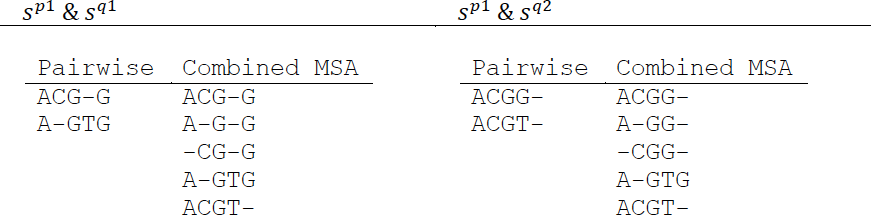
\includegraphics[width=0.9 \textwidth]{fig09/pair_guided_progress_alignment.png}
\end{figure}

%
% NEWPAGE
%
\newpage

%
% Exercise \thesection.2
%
\subsubsection*{Exercise \thesection.2}
Combine two alignments $\mathcal{A}^p$ and $\mathcal{A}^q$ by using the pair-guided approach.

\begin{table}[H]
\centering
\begin{tabular}{lllllll}
$\mathcal{A}^{p}$ & & \hspace{10em} & $\mathcal{A}^{q}$  & &  \\
 & $s^{p1}$: & \verb|TCG| &  &  & $s^{q1}$: & \verb|T-G| \\
                        & $s^{p2}$: & \verb|-CG| &      &                         & $s^{q2}$: & \verb|ACG| \\
                        & $s^{p3}$: &  \verb|T-C| &      &                         &  & 
\end{tabular}
\end{table}

\begin{enumerate}
\item Use the alignment between $s^{p3}$ and $s^{q2}$.

\begin{table}[H]
\centering
\begin{tabular}{ll}
 $s^{p3}$:& \verb|T-C-| \\
 $s^{q2}$:& \verb|-ACG|
\end{tabular}
\end{table}

\end{enumerate}
\bigskip 

%\end{document}

%\documentclass[12pt]{article}
%\usepackage[a4paper, margin=1in]{geometry} 
%\usepackage{graphicx} 
%\usepackage{hyperref}
%\usepackage{float}
%\usepackage{multicol}
%\usepackage{multirow}
%\usepackage{amsmath}
%\usepackage{amssymb}
%\usepackage[ruled]{algorithm2e}
%\usepackage[font=small, labelfont=bf]{caption}
%
%\begin{document}

%
% CLUSTAL
%
\subsection{CLUSTAL}
CLUSTAL W is the most widely used progressive alignment program.

%
% Original version (CLUSTAL)
%
\subsubsection*{Original version (CLUSTAL)}
\begin{itemize}
\item Pairwise alignment between all sequence pairs
\item Phylogenic tree by UPGMA
\item Guided by phylogenetic tree
\item Align by consensus sequences
\end{itemize}

%
% CLUSTAL W
%
\subsubsection*{CLUSTAL W}
\begin{itemize}
\item Phylogenic tree by Neighbor-joining
\item Align by profiles
\end{itemize}

%
% Gap penalty
%
\subsubsection*{Gap penalty}
\begin{itemize}
\item Open
\item Extend
\item End
\item Separation
\end{itemize}

%
% Web version
%
\subsubsection*{Web version}
\begin{itemize}
\item \url{http://www.ch.embnet.org/software/ClustalW.html}
\end{itemize}

\bigskip 

%\end{document}


\end{document}
